\section{Multi-axial Stress States of Circular CFST member}


\subsection{Multi-axial Stress States}

When the CFST members were under loading, composite effects were introduced due to the interaction between concrete core and steel tube. Thus, both the concrete and steel are under multi-axial stress state.

Regarding the concrete, the steel tube will provide confined stress to it and make the material under tri-axial stress state, which is called concrete confinement effect. The strength and the ductility of the concrete is improved by the confinement effect. There were many researchers had studied the concrete confinement effect for CFST members ().

Not only concrete core, but also the steel tube is under multi-axial stress state. The steel tube will provide the confined stress to the concrete core and introduce the confinement effect. In turn, the concrete will expand under axial stress and cause the circumferential stress (or called hoop stress) around the steel tube. As the thickness of the steel tube is relatively small compared to the section diameter, the steel tube could be considered as a 2D shell and the material is under bi-axial stress state (\cite{RN31}). \autoref{fig:steel_biaxial_stress} shows the stress state of the steel tube of circular CFST member. Since the member is under bending force, part of the steel tube is under compression and part of it is under tension. The influences of bi-axial stress state on the steel material properties in the compression and tension areas are different. As can be seen in \autoref{fig:steel_biaxial_stress}, for the compression area, the steel is combined with compressive stress on vertical direction and tensile stress on the horizontal direction. While for the tension area, the steel is under tensile stress at both vertical and horizontal directions.
\begin{figure}[h!]
  \centering
  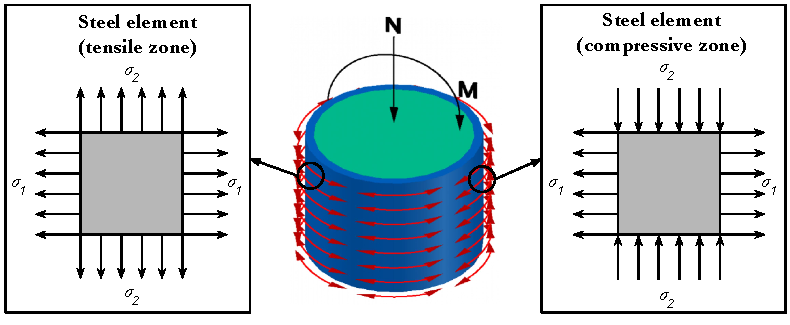
\includegraphics[width=\linewidth]{Figures/Hoop_Stress.pdf}
  \caption{Steel bi-axial stress state under bending force}
  \label{fig:steel_biaxial_stress}
\end{figure}


To consider the yield stress of steel under bi-axial stress state, the yield surface is introduced (\autoref{fig:von_mises}). It should be noted that, positive value stands for tensile stress whilst negative value presents compressive stress. The hoop stress (\(\sigma_h\)) is plotted at the positive \(x\) axis and the corresponding steel yield stresses under compression (\(f_{yc}\)) and tension (\(f_{yt}\)) are annotated on the yield surface. It could be found that, for steel at compression area, the compressive yield stress is smaller than the uni-axial yield stress (\(f_{y}\)), which will have negative influence on the CFST member capacity. On the contrary, the steel yield stress at tension area will be larger than the uni-axial yield stress, which would benefit the member strength under bending. For circular CFST member under pure compression loading, the whole steel section is under compression and the yield stress of the steel is reduced from (\(f_{y}\)) to (\(f_{yc}\)), Therefore, the steel bi-axial stress has negative influence on the CFST column�s compressive resistance capacity. But for the bending capacity of CFST member, the influence of the steel bi-axial stress state depends on the relative area between the compression part and tension part, since the bi-axial stress state can increase yield stress under tension and reduce yield stress under compression. Thus, if the tensile area of the steel section is larger than the compressive, the steel bi-axial stress will benefit the bending resistance capacity of the CFST members and vice versa.
\begin{figure}[h!]
    \centering
    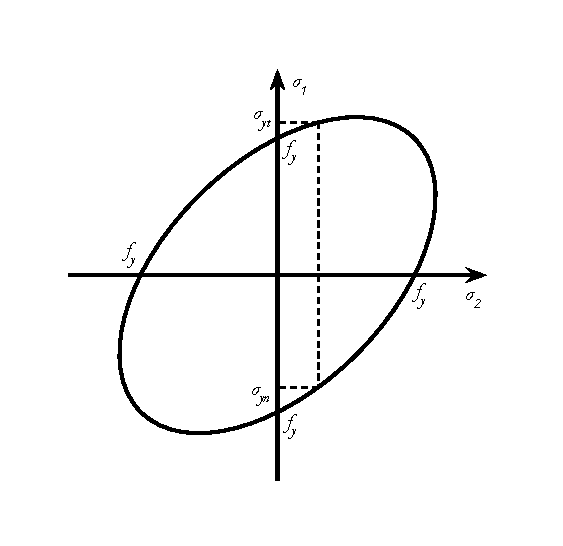
\includegraphics[width=0.75\linewidth]{Figures/Von_Mises.pdf}
    \caption{Steel yield surface}
    \label{fig:von_mises}
\end{figure}


\subsection{Influence of Multi-axial stress state on Bending Capacity}

As the concrete confinement effect and the steel tensile yield stress can improve the bending capacity while the steel tensile yield stress will decrease the bending capacity of circular specimens. To investigate if the combination of the multi-axial stress states have either positive or negative influence on the bending capacity of circular CFST columns, both experimental and numerical studies had been carried out. 

Experimental tests, which were detailed in \cite{Silva2016}, had been conducted to study characterize the bending behaviour of the circular CFST columns under flexural loading. Based on the test results, two numerical models, namely a 3D Finite Element (FE) model and a Distributed Plasticity (DP) model had been proposed to simulate the bending behaviour of circular CFST members. The details of the two numerical models, including the member geometry, the steel-concrete interaction and the material properties, could be found in \cite{Jiang2018}. The 3D model has the possibility to consider the multi-axial stress states of the two materials, since the solid/shell elements were used. While for the DP model, the multi-axial stress state could not be considered as the fibre section could only consider the uni-axial material properties. Thus, the influence of multi-axial stress states on the bending capacity of circular CFST member could be investigated by comparing the predicted results of DP model with the test data.

The lateral load versus drift ratio plots comparison between the experimental and the predicted are plotted in \autoref{fig:test_vs_FE}. It should be noted that, the drift ratio ($\theta$) is defined as the ratio between specimen top lateral displacement and the specimen test length. It could be observed that, the DP model could predict accurate elastic stiffness of CFST members. But regarding the plastic behaviour, the lateral resistances given by the DP model were always lower than the test results. Considering that the DP model could not consider the multi-axial stress state, it could be concluded that, combination of multi-axial stress states could benefit the bending behaviour of the circular CFST member under bending combined with moderate constant axial load. 
\begin{figure}[h!]
    \centering
    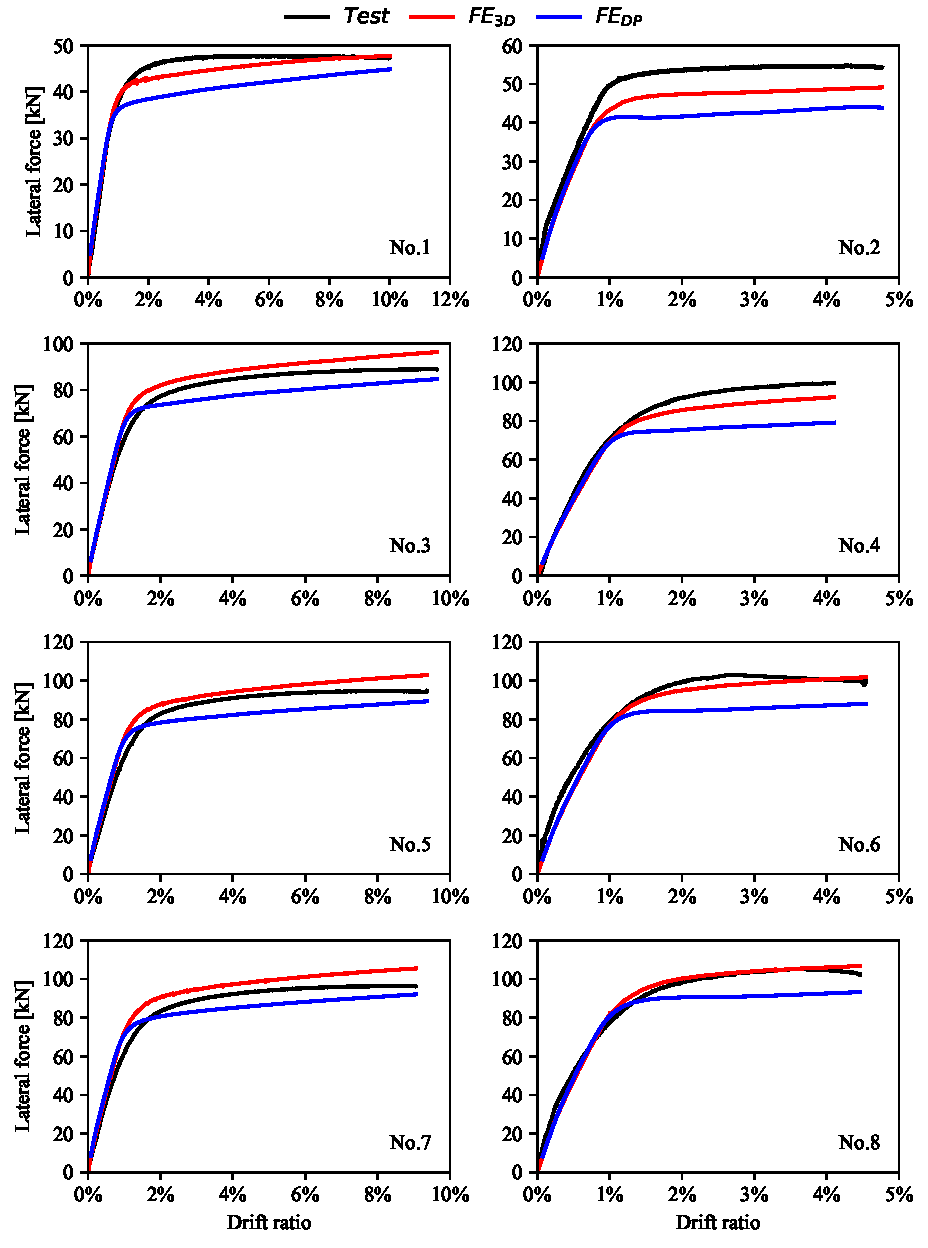
\includegraphics[width=\linewidth]{Figures/Test_vs_FE.pdf}
    \caption{Lateral load versus drift ratio plots comparison between test results, 3D FE model and DP model}
    \label{fig:test_vs_FE}
\end{figure}

Regarding the 3D FE model, good agreement is found by comparing its prediction with test results. It proves that, the 3D model could capture the influence of multi-axial load stress state. To further verify the fact, the vertical stress versus vertical strain curves around the steel tube was plotted, as shown in Figure \ref{fig:hoop_stress_FE}. As a reference curve, the uni-axial stress/strain curve of steel model had also been plot in the same figure. The tensile stress/strain was defined as positive value, while the compressive stress/strain were defined as negative value. It could be seen that, the compressive yield stress are less than the uni-axial stress and vice versa, which is in line with the conclusion obtained from the yield surface. Thus, it enhances the fact that, the 3D FE model could capture the multi-axial stress states. 
\begin{figure}[h!]
    \centering
    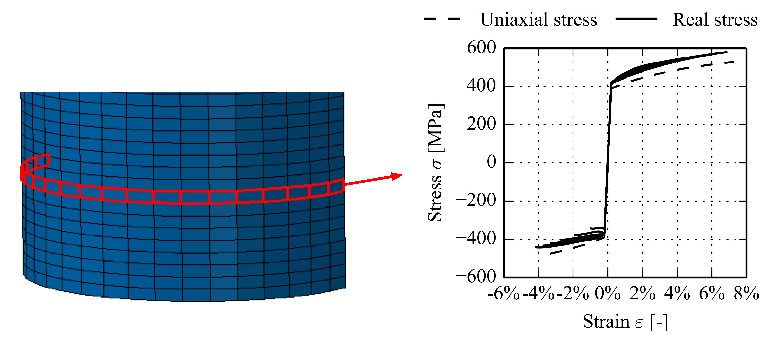
\includegraphics[width=\linewidth]{Figures/Hoop_Stress_FE.pdf}
    \caption{The vertical stress/strain plots output from the 3D FE model}
    \label{fig:hoop_stress_FE}
\end{figure}

\subsection{Previous Study on Multi-axial Stress State Influence}

In the past, there were many researchers had carried out the studies on prediction of concrete confined stress (Han et al. [2001], Hu et al. [2003], Hu et al. [2005] and Tort and Hajjar [2010]). But in these researches, the influence of steel bi-axial stress state was ignored. Therefore, the derived confined concrete properties by these studies may lead to deviation.

Lai and Varma [2016] had performed parametric study on CFST members under compressive loading with the consideration of multi-axial stress states influences on both concrete and steel. The equation to calculate the confined concrete strength had been derived. Besides that, the steel compressive yield strength was reduced to $0.9f_y$. But regarding the tensile steel yield stress, there was no correction. Thus, the proposed 
 material strength correction equations of Lai and Varma [2016] were suitable for CFST member subjected to axial compression but not for bending. 

Fujimoto et al. [2004] and Inai et al. [2004] had used the DP model to predict the bending behaviour of CFST members. To consider the influences of multi-axial stress states, they combined the previous researches on concrete confined stress and steel bi-axial yield stress (Kato and Nishiyama [1980], Sakino and Sun [1994], Nakahara et al. [1999] and Sakino et al. [1998]) and summarized the material strength correction equations for both concrete and steel strength. For circular CFST members, the confined concrete strength was given in Equations (\ref{eq:Sakino_1}) - (\ref{eq:Sakino_2}).
\begin{equation}
    f_{cc} = f_c + 4.1\sigma_r
    \label{eq:Sakino_1}
\end{equation}
\begin{equation}
    \sigma_r = \frac{0.38tf_y}{D - 2t}
    \label{eq:Sakino_2}
\end{equation}

In the studies, a hoop stress of $0.19f_y$ had been assumed and the steel bi-axial yield stress under compression and tension had been adopted as $0.91f_y$ and $1.08f_y$, respectively. To verify the accuracy of the material strength correction equations, the DP models were re-analysed with the corrected material strength. \autoref{tb:sakino} shows the confined concrete strength and the steel bi-axial yield stresses. 
\begin{table}[h!]
  \caption{The corrected material strength for the circular CFST specimens}
  \centering

  \begin{tabular} {*{10}{| c} |}
    \hline
    \multirow{2}{*}{No.}   & \multirow{2}{*}{Specimen Name}    & $D$     & $t$    & $P$    & $f_c$    & $f_y$  & $f_{cc}$    & $f_{yt}$    & $f_{yt}$ \\

        &  & [mm]     & [mm]    & [kN]    & [MPa]    & [MPa]  & [MPa]    & [MPa]    & [MPa] \\
    \hline

    \input{Tables/Table_Sakino.txt}

    \iffalse
    1 & CR-RuC15\%-219-3-0\%-M & 219 & 2.8 & 0 & 20 & 309 & 25 & 281 & 334 \\
    \hline
    2 & CR-RuC15\%-219-3-15\%-M & 219 & 2.8 & 222 & 20 & 309 & 25 & 281 & 334 \\
    \hline
    3 & CR-RuC15\%-219-5-0\%-M & 219 & 4.7 & 0 & 20 & 393 & 32 & 358 & 424 \\
    \hline
    4 & CR-RuC15\%-219-5-15\%-M & 219 & 4.7 & 290 & 20 & 393 & 32 & 358 & 424 \\
    \hline
    5 & CR-RuC5\%-219-5-0\%-M & 219 & 4.7 & 0 & 39 & 393 & 49 & 358 & 424 \\
    \hline
    6 & CR-RuC5\%-219-5-15\%-M & 219 & 4.7 & 359 & 39 & 393 & 49 & 358 & 424 \\
    \hline
    7 & CR-StdC-219-5-0\%-M & 219 & 4.7 & 0 & 53 & 393 & 62 & 358 & 424 \\
    \hline
    8 & CR-StdC-219-5-15\%-M & 219 & 4.7 & 393 & 53 & 393 & 62 & 358 & 424\\
    \fi
    \hline
  \end{tabular}
  \label{tb:sakino}
\end{table}

\autoref{fig:Sakino_verification} displayed the lateral load versus drift ratio curves comparison of three results, namely the tests results, the DP model results with uni-axial material strength and the DP model results with corrected material strength. The 4 plots on the left column belongs to the specimens with no axial load. It could be found that, with the correction methods given by Fujimoto et al. [2004] and Inai et al. [2004], the accuracy of the DP model had been improved, as good agreements were found between corrected DP model and the test results. But regarding the specimens with constant axial loads (plots on the right column), no improvement was found of the corrected DP model compared to the original DP model. As the constant factors were used to corrected the steel bi-axial stress, it could be summarized that the steel bi-axial stress should depends on the axial load level.
\begin{figure}[h!]
    \centering
    \includegraphics[width=\linewidth]{Figures/Sakino_Comparison.pdf}
    \caption{Lateral load versus drift ratio plots comparison between test results, DP model and the corrected DP model}
    \label{fig:Sakino_verification}
\end{figure}

As the aforementioned material strength correction methods were proved to be in-accurate for circular CFST columns under bending combined with constant axial loads, It is necessary to propose new material strength correction methods for both concrete and steel.
